\documentclass[11pt,a4paper]{article}
\usepackage[spanish,es-nodecimaldot]{babel}	% Utilizar español
\usepackage[utf8]{inputenc}					% Caracteres UTF-8
\usepackage{graphicx}						% Imagenes
\usepackage[hidelinks]{hyperref}			% Poner enlaces sin marcarlos en rojo
\usepackage{fancyhdr}						% Modificar encabezados y pies de pagina
\usepackage{float}							% Insertar figuras
\usepackage[textwidth=390pt]{geometry}		% Anchura de la pagina
\usepackage[nottoc]{tocbibind}				% Referencias (no incluir num pagina indice en Indice)
\usepackage{enumitem}						% Permitir enumerate con distintos simbolos
\usepackage[T1]{fontenc}					% Usar textsc en sections
\usepackage{amsmath}						% Símbolos matemáticos
\usepackage{listings}
\usepackage{color}

 
\definecolor{codegreen}{rgb}{0,0.6,0}
\definecolor{codegray}{rgb}{0.5,0.5,0.5}
\definecolor{codepurple}{rgb}{0.58,0,0.82}
\definecolor{backcolour}{rgb}{0.99,0.99,0.99}
 
\lstdefinestyle{mystyle}{
    backgroundcolor=\color{backcolour},   
    commentstyle=\color{codegreen},
    keywordstyle=\color{magenta},
    numberstyle=\tiny\color{codegray},
    stringstyle=\color{codepurple},
    basicstyle=\footnotesize,
    breakatwhitespace=false,         
    breaklines=true,                 
    captionpos=b,                    
    keepspaces=true,                 
    numbers=left,                    
    numbersep=5pt,                  
    showspaces=false,                
    showstringspaces=false,
    showtabs=false,                  
    tabsize=2
}
 
\lstset{style=mystyle, language=Java}

% Comando para poner el nombre de la asignatura
\newcommand{\asignatura}{Técnicas de los Sistemas Inteligentes}
\newcommand{\autor}{José María Sánchez Guerrero}
\newcommand{\titulo}{Práctica 1}
\newcommand{\subtitulo}{Desarrollo de un agente basado en búsqueda}

% Configuracion de encabezados y pies de pagina
\pagestyle{fancy}
\lhead{\autor{}}
\rhead{\asignatura{}}
\lfoot{Grado en Ingeniería Informática}
\cfoot{}
\rfoot{\thepage}
\renewcommand{\headrulewidth}{0.4pt}		% Linea cabeza de pagina
\renewcommand{\footrulewidth}{0.4pt}		% Linea pie de pagina

\begin{document}
\pagenumbering{gobble}

% Pagina de titulo
\begin{titlepage}

\begin{minipage}{\textwidth}

\centering

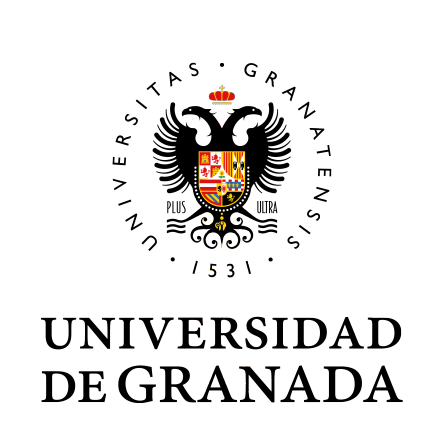
\includegraphics[scale=0.5]{img/ugr.png}\\

\textsc{\Large \asignatura{}\\[0.2cm]}
\textsc{GRADO EN INGENIERÍA INFORMÁTICA}\\[1cm]

\noindent\rule[-1ex]{\textwidth}{1pt}\\[1.5ex]
\textsc{{\Huge \titulo\\[0.5ex]}}
\textsc{{\Large \subtitulo\\}}
\noindent\rule[-1ex]{\textwidth}{2pt}\\[3.5ex]

\end{minipage}

\vspace{0.5cm}

\begin{minipage}{\textwidth}

\centering

\textbf{Autor}\\ {\autor{}}\\[2.5ex]
\textbf{Rama}\\ {Computación y Sistemas Inteligentes || Grupo 2 - Pablo Mesejo}\\[2.5ex]
\vspace{0.3cm}


\includegraphics[scale=0.3]{img/etsiit.jpeg}

\vspace{0.7cm}
\textsc{Escuela Técnica Superior de Ingenierías Informática y de Telecomunicación}\\
\vspace{1cm}
\textsc{Curso 2019-2020}
\end{minipage}
\end{titlepage}

\pagenumbering{arabic}
\tableofcontents
\thispagestyle{empty}				% No usar estilo en la pagina de indice

\newpage

\setlength{\parskip}{1em}


\section{Introducción}

La práctica consiste en implementar varios agentes que se puedan desenvolver adecuadamenete en los
distintos escenarios propuestos. Dispondremos de 5 mapas distintos, cada uno de ellos con un escenario
distinto.

\begin{itemize}
    \item En el primero simplemente tendremos que encontrar la salida
    \item En el segundo hay que recoger 10 gemas y luego salir
    \item En el tercero aguantar 2000 ticks del juego sin morir con un enemigo
    \item El cuarto aguantar 2000 ticks con varios enemigos
    \item El último será una fusión entre todos los otros, ya que hay que recoger 10 gemas y salir sin
          ser atrapado por ningun enemigo.
\end{itemize}

En mi caso he utilizado un algoritmo IDA* para encontrar los caminos más óptimos, y una técnica reactiva
que consiste en mantener al avatar lo más alejado posible de los enemigos en cada tick.


\section{Deliberativo}

Para nuestros agentes deliberativos vamos a utilizar, como hemos mencionado antes, el algoritmo IDA*.
Este algoritmo está basado en el algoritmo base A* (es una extensión de este), sin embargo, he decidido
implementar este ya que obtiene los mismos resultados, pero no almacena todos los posibles nodos que puede
visitar y reduce considerablemente el consumo de memoria.

A la hora de implementarlo, he necesitado dos clases. La primera es la clase ''\textbf{\textit{IDAStar.java}}'',
en la cual está implementado todo el algoritmo; y otra llamada ''\textbf{\textit{Node.java}}'', la cual
utilizamos para representar de una forma más sencilla cada una de las casillas del tablero adaptadas a nuestro
algoritmo. A continuación vamos a detallar sus implementaciones.

Empecemos con la clase \textit{Node} ya que la usaremos dentro de la otra. Lo primero es la declaración de
variables a utilizar:
\newline
\begin{lstlisting}
    // Valor heuristico del nodo actual
    private double hScore = Double.MIN_VALUE;
    // Coste del camino recorrido
    private double gScore = 0.0;
    // La suma de los valores anteriores
    private double fScore = 0.0;

    // Padre del nodo actual
    private Node parent;
    // Posicion en coordenadas (x,y) del nodo actual
    private Vector2d position;
\end{lstlisting}

He añadido un constructor para poder crear un nuevo nodo a partir de una posición (x,y):
\newline
\begin{lstlisting}
    /**
	 * Constructor a partir de una posicion (x,y) del mapa.
	 * 
	 * @param position
	 */
	Node(Vector2d position){
		this.position = position;
	}
\end{lstlisting}

Para acceder y modificar estas variables tendremos sus correspondientes métodos \textit{getX} y \textit{setX}.
Para compara un nodo con otro, es decir, comparar los valores de \textit{f()}, he añadido la siguiente función:
\newline
\begin{lstlisting}
    /**
     * Compara el valor de f() del nodo actual con otro.
     * 
     * @param n Nodo a comparar.
     * @return -1 si el actual es menor que n,
     *          0 si actual es igual que n,
     *          1 si actual es mayor que n.
     */
    @Override
    public int compareTo(Node n) {
        if(this.fScore < n.fScore)
            return -1;
        if(this.fScore > n.fScore)
            return 1;
        return 0;
    }
\end{lstlisting}

También dispondremos de una función que determina si un nodo es igual que otro, pero no en cuanto a sus valores
de \textit{f()}, si no en cuanto a sus estados:
\newline
\begin{lstlisting}
    /**
     * Determina si otro nodo es igual al nodo actual. Dos nodos son
     * iguales si sus estados son iguales (no f ()).
     * 
     * @param otro nodo Nodo a comparar.
     * @return true si el otro nodo es igual, false en caso contrario.
     */
    @Override
    public boolean equals(Object o)
    {
        return this.position.equals(((Node)o).position);
    }
\end{lstlisting}

Para obtener los nodos sucesores he utilizado la siguiente función:
\newline
\begin{lstlisting}
    /**
     * Genera una lista de los nodos sucesores al nodo actual.
     * Devolvemos cada una de las casillas que rodean a la actual,
     * comprobando antes que esta casilla sea transitable, es
     * decir, no sea un obstaculo.
     *
     * @param tiposObs son las casillas no transitables del mapa.
     * @return lista de nodos sucesores.
     */
   public List<Node> getSuccessors(ArrayList<Vector2d> tiposObs){

       // Declaromos una lista para los nodos
       List<Node> successors = new ArrayList<Node>();
       
       // Insertamos en ella las casillas que rodean a la actual
       Node top = new Node(new Vector2d(this.position.x,
                                        this.position.y-1));
       top.setParent(this);
       Node bottom = new Node(new Vector2d(position.x, position.y+1));
       bottom.setParent(this);
       Node left = new Node(new Vector2d(position.x-1, position.y));
       left.setParent(this);
       Node right = new Node(new Vector2d(position.x+1, position.y));
       right.setParent(this);
       
       // Comprobamos que no son casillas no transitables
       if (!tiposObs.contains( top.position )) {
           successors.add(top);
       }
       if (!tiposObs.contains( bottom.position )) {
           successors.add(bottom);
       }
       if (!tiposObs.contains( left.position )) {
           successors.add(left);
       }
       if (!tiposObs.contains( right.position )) {
           successors.add(right);
       }
       
       return successors;
   }
\end{lstlisting}

Por último, tenemos la función que determina la \textit{h()}. Como estamos en un mapa cuadriculado, la distancia
al padre siempre va a ser 1, por tanto:
\newline
\begin{lstlisting}
    /**
     * Devuelve la distancia entre el nodo actual y el padre.
     *
     * @return 1, porque estamos en un mapa cuadriculado.
     */
    public double distFromParent() {
    	return 1;
    }
\end{lstlisting}

Una vez hemos terminado con la clase \textit{Node}, vamos a pasar a la clase \textbf{\textit{IDAStar}}



\subsection{Deliberativo simple}

\subsection{Deliberativo compuesto}



\newpage

\section{Reactivo}

\subsection{Reactivo simple}

\subsection{Reactivo compuesto}



\newpage

\section{Deliberativo-Reactivo}


\end{document}